\subsection{不同玻璃类型风化组与无风化组的化学成分差异}

\subsubsection{数据分组与预处理}

附件表单~2 共包含 69 个化学成分采样点。按照题目给出的有效性标准，
将成分总和不在 $85\%\sim105\%$ 范围内的 15 号和 17 号采样点剔除，
最终保留 67 个有效采样点。对于未检出的化学成分，以 0 记录；随后将每个
有效采样点的 14 种化学成分归一化至总和为 $100\%$，以消除不同样本总量
差异对组间比较的影响。

为避免玻璃类型的混杂作用，本文不直接混合高钾玻璃与铅钡玻璃，而是在
两类玻璃内部，按照采样点实际风化状态分别构造风化组与无风化组。高钾
玻璃包括 12 个无风化采样点和 6 个风化采样点；铅钡玻璃包括 23 个无风化
采样点和 26 个风化采样点。

\subsubsection{统计方法的选择}

部分化学成分含有较多零值，分布具有明显偏态；同时，高钾玻璃风化组仅有
6 个样本，难以保证独立样本 $t$ 检验所要求的近似正态性。因此，本文首先
利用箱线图比较两组数据的中位数、四分位距和离散程度，再采用对总体分布
形式要求较低的 Mann--Whitney $U$ 检验，对同一玻璃类型下风化组与无风化
组的成分分布进行比较。

对于每一种化学成分，建立假设
\begin{equation}
    \begin{aligned}
        H_0 &: \text{风化组与无风化组的总体分布不存在系统差异},\\
        H_1 &: \text{风化组与无风化组的总体分布存在系统差异}.
    \end{aligned}
\end{equation}

设风化组和无风化组样本量分别为 $n_1$ 和 $n_2$，以风化组对应的
$U$ 统计量计算秩二列效应量
\begin{equation}
    r_{\mathrm{rb}}=\frac{2U}{n_1n_2}-1.
\end{equation}
其中，$r_{\mathrm{rb}}>0$ 表示风化组的取值整体偏高，
$r_{\mathrm{rb}}<0$ 表示风化组的取值整体偏低，
$|r_{\mathrm{rb}}|$ 越大表示两组分布分离程度越明显。

两类玻璃各检验 14 种化学成分，共进行 $m=28$ 次比较。为控制多重检验
产生的假阳性，本文对原始 $p$ 值实施 Benjamini--Hochberg 校正。将原始
$p$ 值从小到大排列为 $p_{(1)},\ldots,p_{(m)}$，相应校正值为
\begin{equation}
    q_{(i)}=\min_{j\geq i}\left\{\frac{m}{j}p_{(j)}\right\},
\end{equation}
并以 $q<0.05$ 作为差异显著的判断标准。

\subsubsection{箱线图分析}

高钾玻璃中，风化组二氧化硅的整体分布明显高于无风化组；氧化钾、
氧化镁、氧化铝和五氧化二磷的分布则整体偏低，如图~\ref{fig:q1b-high-k}
所示。二氧化硅和氧化钾的两组分离最为明显。氧化钙、氧化铁和氧化铅
也呈现下降趋势，但两组样本仍有一定重叠。

\begin{figure}[H]
    \centering
    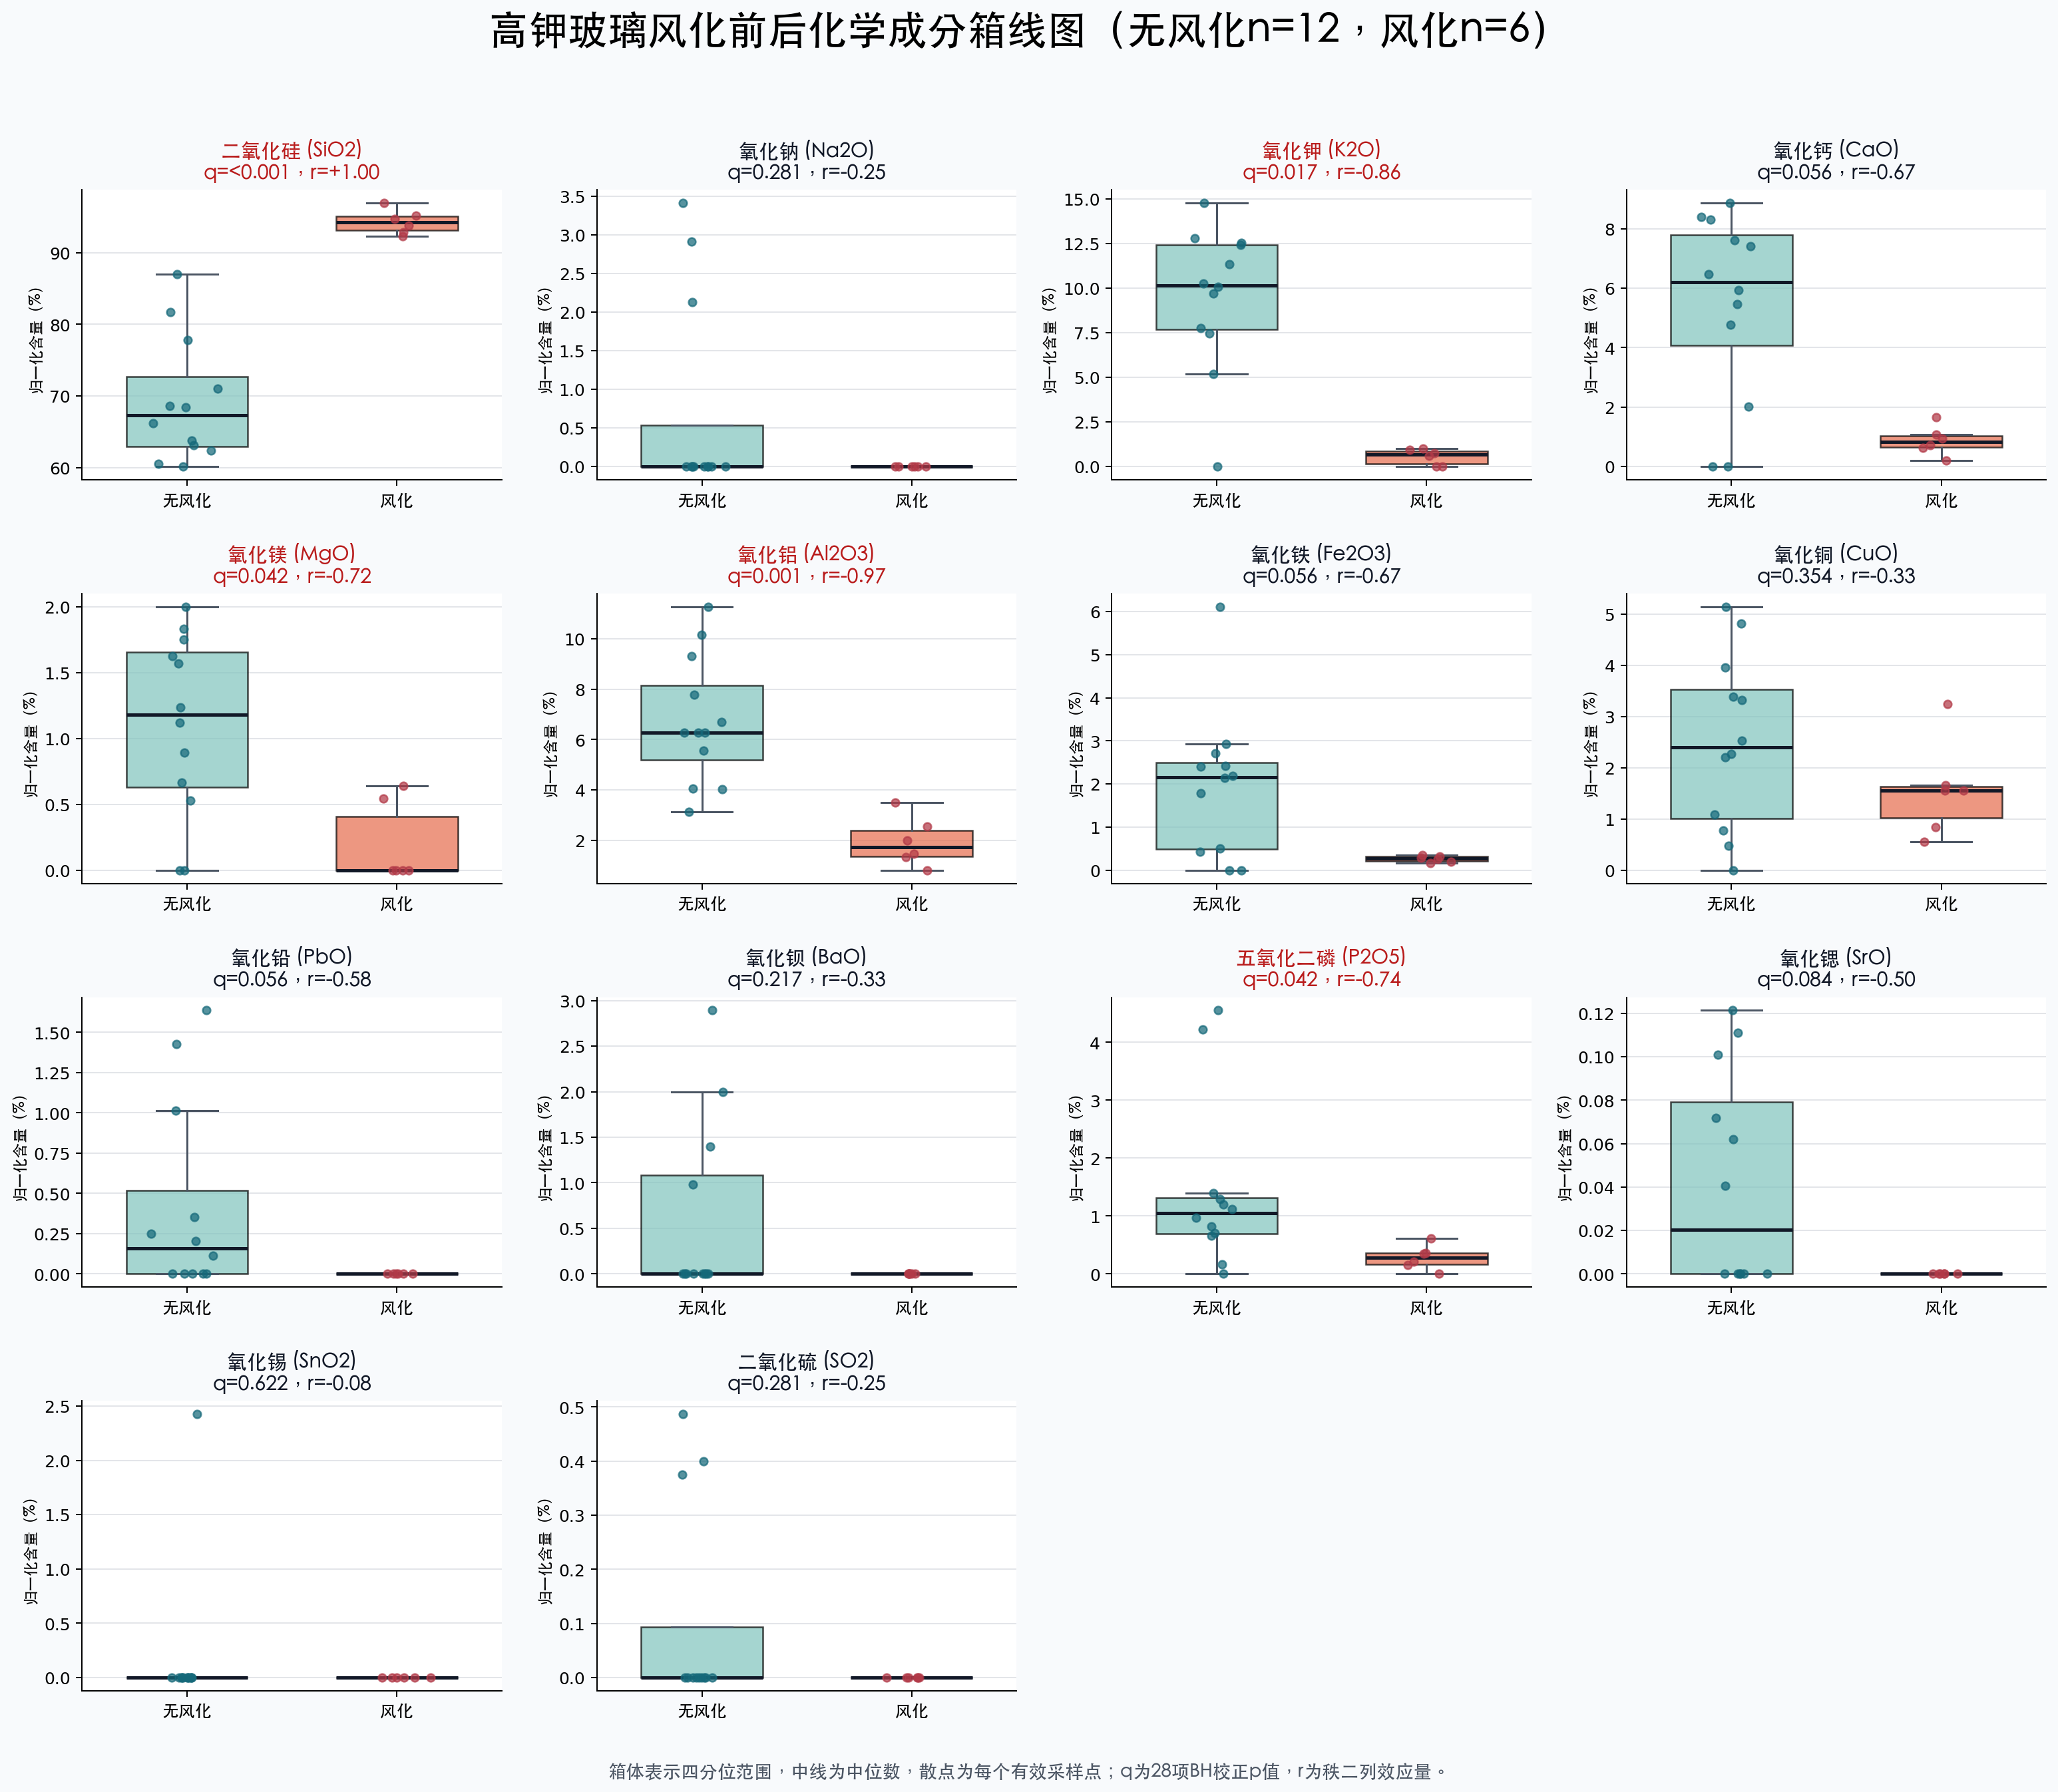
\includegraphics[width=0.96\textwidth]{figures/q1b_high_k_boxplot.png}
    \caption{高钾玻璃风化组与无风化组的化学成分箱线图}
    \label{fig:q1b-high-k}
\end{figure}

铅钡玻璃中，风化组二氧化硅的整体分布明显低于无风化组，而氧化铅、
氧化钙和五氧化二磷的整体分布较高，如图~\ref{fig:q1b-pbba} 所示。
氧化镁、氧化钾和氧化铁等成分的两组箱体及散点重叠较多，其组间差异
相对较弱。

\begin{figure}[H]
    \centering
    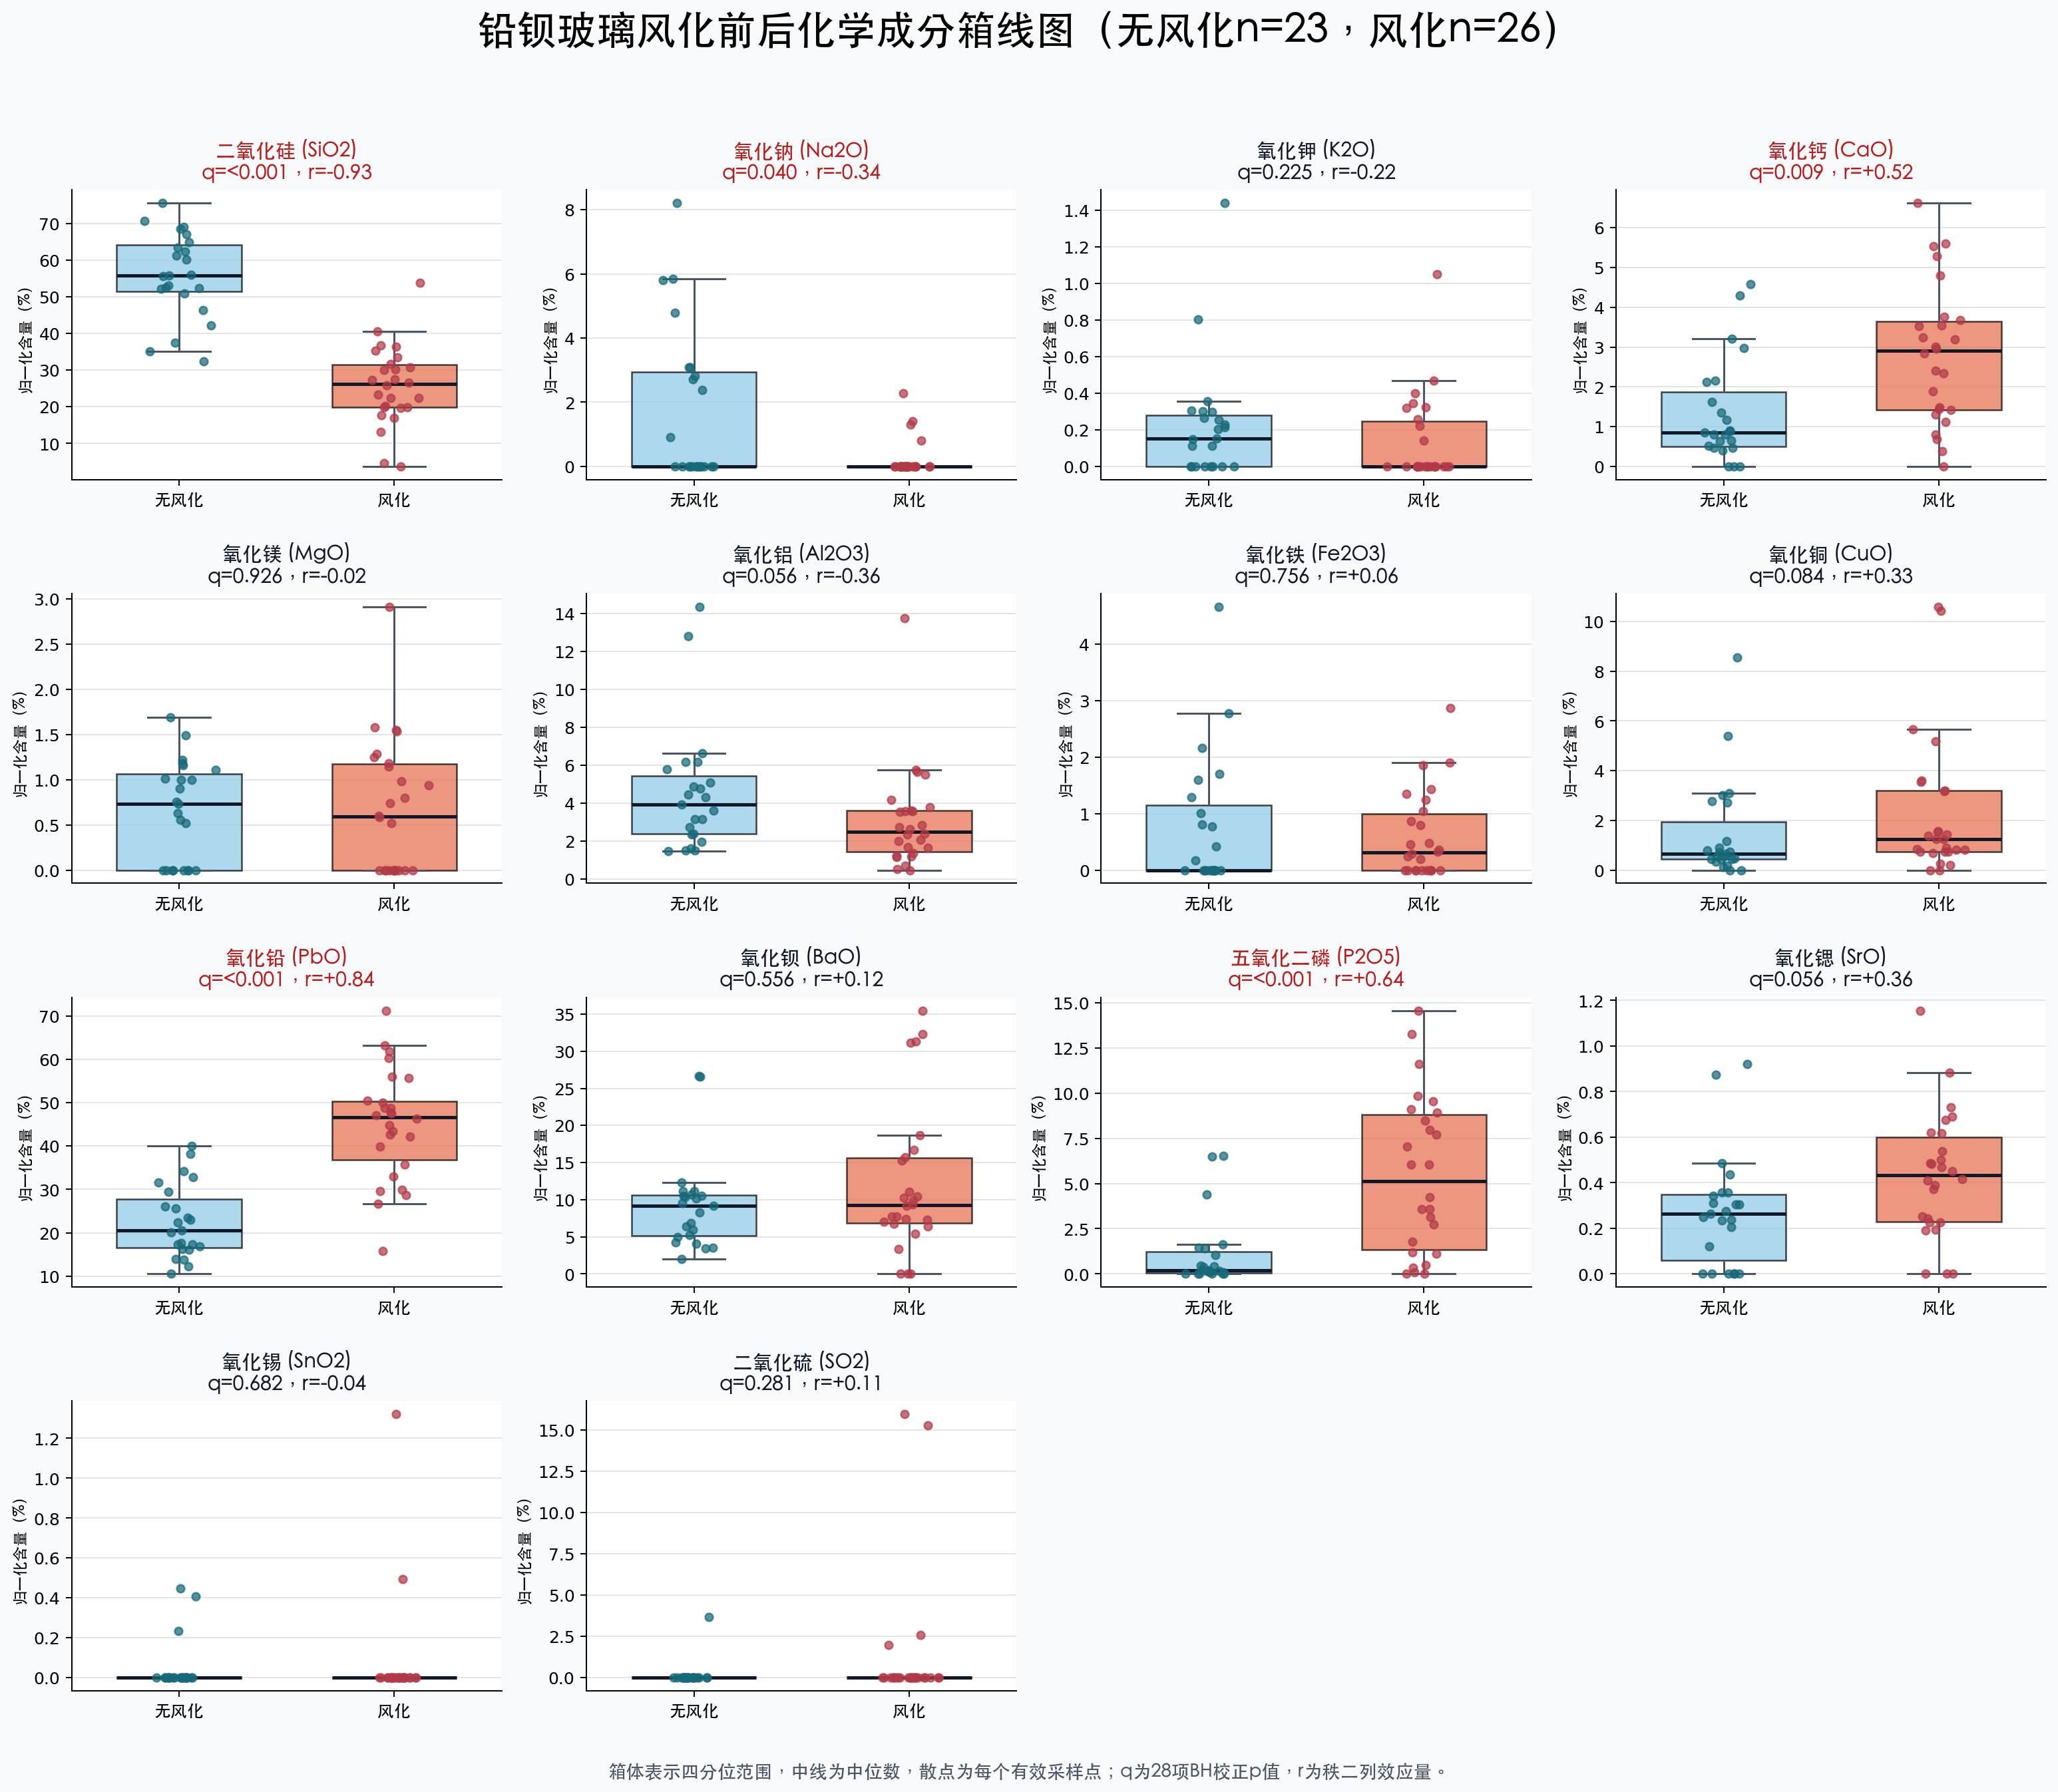
\includegraphics[width=0.96\textwidth]{figures/q1b_pbba_boxplot.png}
    \caption{铅钡玻璃风化组与无风化组的化学成分箱线图}
    \label{fig:q1b-pbba}
\end{figure}

箱线图只能展示样本中的分布差异，不能单独判断这种差异是否足以排除
随机波动。因此，下面结合 Mann--Whitney $U$ 检验、BH 校正和效应量
进行定量判断。

\subsubsection{检验结果与解释}

表~\ref{tab:q1b-high-k} 给出了高钾玻璃经 BH 校正后达到显著水平的
化学成分。风化组二氧化硅相对含量显著较高，且两组样本完全分离
（$q<0.001$，$r_{\mathrm{rb}}=1.00$）；氧化钾、氧化镁、氧化铝和
五氧化二磷相对含量显著较低。氧化钙、氧化铁和氧化铅虽呈下降趋势，
但校正后均为 $q\approx0.056$，未达到 $0.05$ 的显著性标准，故不将其
表述为显著差异。

\begin{table}[H]
    \centering
    \caption{高钾玻璃风化组与无风化组的显著差异成分}
    \label{tab:q1b-high-k}
    \small
    \begin{tabular}{cccccc}
        \toprule
        化学成分 & 风化组方向 & BH 校正 $q$ 值 & $r_{\mathrm{rb}}$ & 效应大小 & 统计结论 \\
        \midrule
        二氧化硅       & 较高 & $<0.001$ & $+1.00$ & 大 & 显著 \\
        氧化钾         & 较低 & $0.017$  & $-0.86$ & 大 & 显著 \\
        氧化镁         & 较低 & $0.042$  & $-0.72$ & 大 & 显著 \\
        氧化铝         & 较低 & $0.001$  & $-0.97$ & 大 & 显著 \\
        五氧化二磷     & 较低 & $0.042$  & $-0.74$ & 大 & 显著 \\
        \bottomrule
    \end{tabular}
\end{table}

铅钡玻璃的显著差异成分如表~\ref{tab:q1b-pbba} 所示。风化组二氧化硅
和氧化钠相对含量显著较低，氧化钙、氧化铅和五氧化二磷相对含量显著较高。
其中，二氧化硅和氧化铅的效应量绝对值最大，说明两组分布的分离最为明显。
氧化铝和氧化锶虽呈一定变化趋势，但其 BH 校正值约为 $0.056$，尚无充分
证据认定其存在显著差异。

\begin{table}[H]
    \centering
    \caption{铅钡玻璃风化组与无风化组的显著差异成分}
    \label{tab:q1b-pbba}
    \small
    \begin{tabular}{cccccc}
        \toprule
        化学成分 & 风化组方向 & BH 校正 $q$ 值 & $r_{\mathrm{rb}}$ & 效应大小 & 统计结论 \\
        \midrule
        二氧化硅       & 较低 & $<0.001$ & $-0.93$ & 大   & 显著 \\
        氧化钠         & 较低 & $0.040$  & $-0.34$ & 中等 & 显著 \\
        氧化钙         & 较高 & $0.009$  & $+0.52$ & 大   & 显著 \\
        氧化铅         & 较高 & $<0.001$ & $+0.84$ & 大   & 显著 \\
        五氧化二磷     & 较高 & $<0.001$ & $+0.64$ & 大   & 显著 \\
        \bottomrule
    \end{tabular}
\end{table}

综上，在现有样本中，两类玻璃呈现不同的风化相关成分特征：高钾玻璃
风化组主要表现为二氧化硅相对含量较高，以及钾、镁、铝、磷相关成分
相对含量较低；铅钡玻璃风化组主要表现为二氧化硅和氧化钠相对含量较低，
而氧化铅、氧化钙和五氧化二磷相对含量较高。由于化学成分属于总和受限
的组成数据，上述“较高”与“较低”均指归一化后的相对含量差异，不应直接
解释为某种元素的绝对增加或流失。此外，部分文物含有多个采样点，本节
结果反映的是采样点层面的统计关联，不能单独作为风化因果效应的证明。
